\item The ECG signal from {\tt BME354L\_CANINE\_ECG.mat} is shown below:

\begin{center}
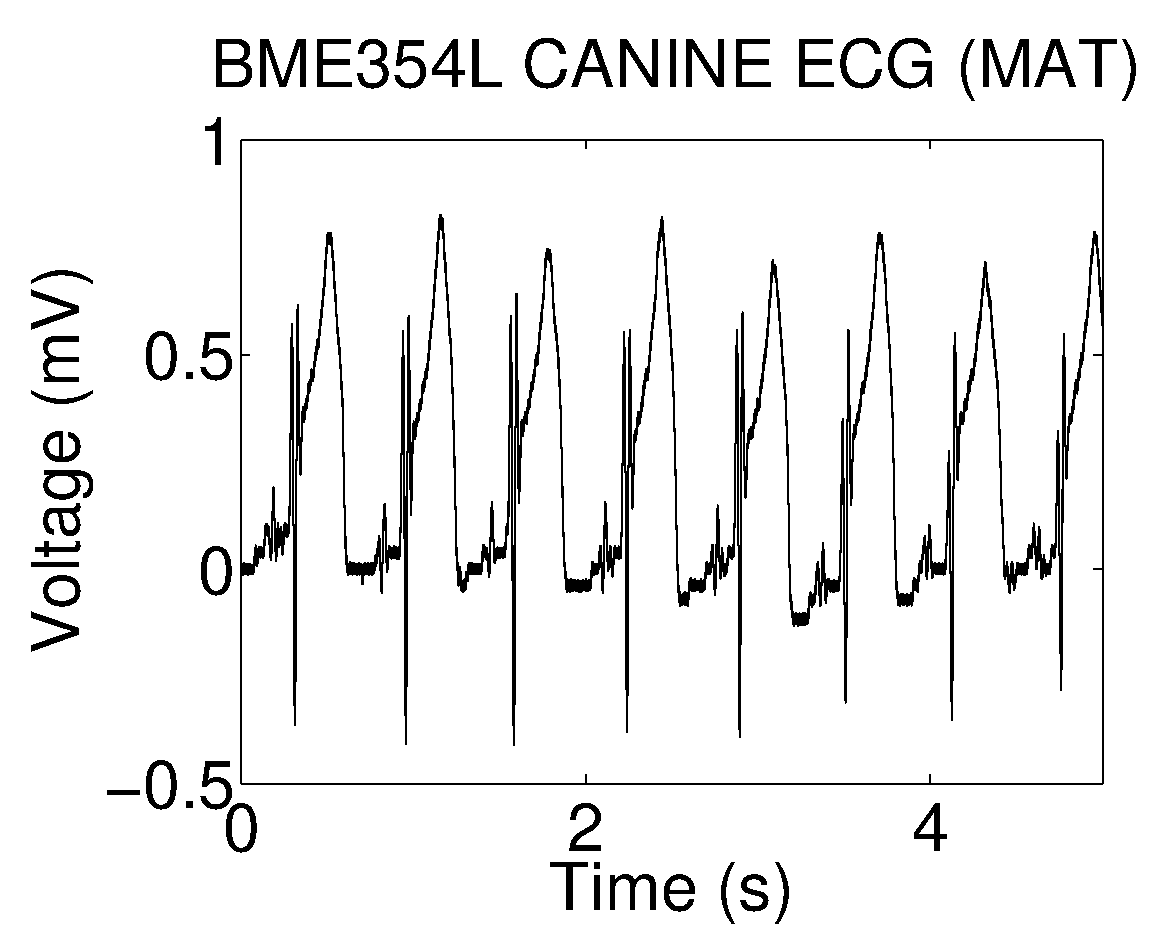
\includegraphics[width=0.5\linewidth]{ecg_data/ecg_mat.eps}
\end{center}

The range of the signal is $\sim$-4.1--0.83 mV (1.24
mV relative range); the noise is $\sim \pm$0.035 mV based on estimation from the
temporal ranges where signal is not expected (average value between T-P
intervals).


Based on the signal and noise voltage ranges, we can sample our signal
voltage range with noise as the limiting factor as $\frac{1.24 mV}{0.07 mV}$ =
17.7.  Four bits will give me 16 discrete levels, which I will assume is
adequate for a minimum value; going to 5 bits would give me 32, which would be
better, though more noise will get captured.

Assuming 4-bit digital representation, $V_\textrm{LSB}$ = 77.5 $\mu$V.

The sampling frequency of the data can be found as {\tt mean(diff(t))}$^{-1}$ = 20 kHz.

The ECG signal from {\tt BME354L\_CANINE\_ECG.dat} is shown below:

\begin{center}
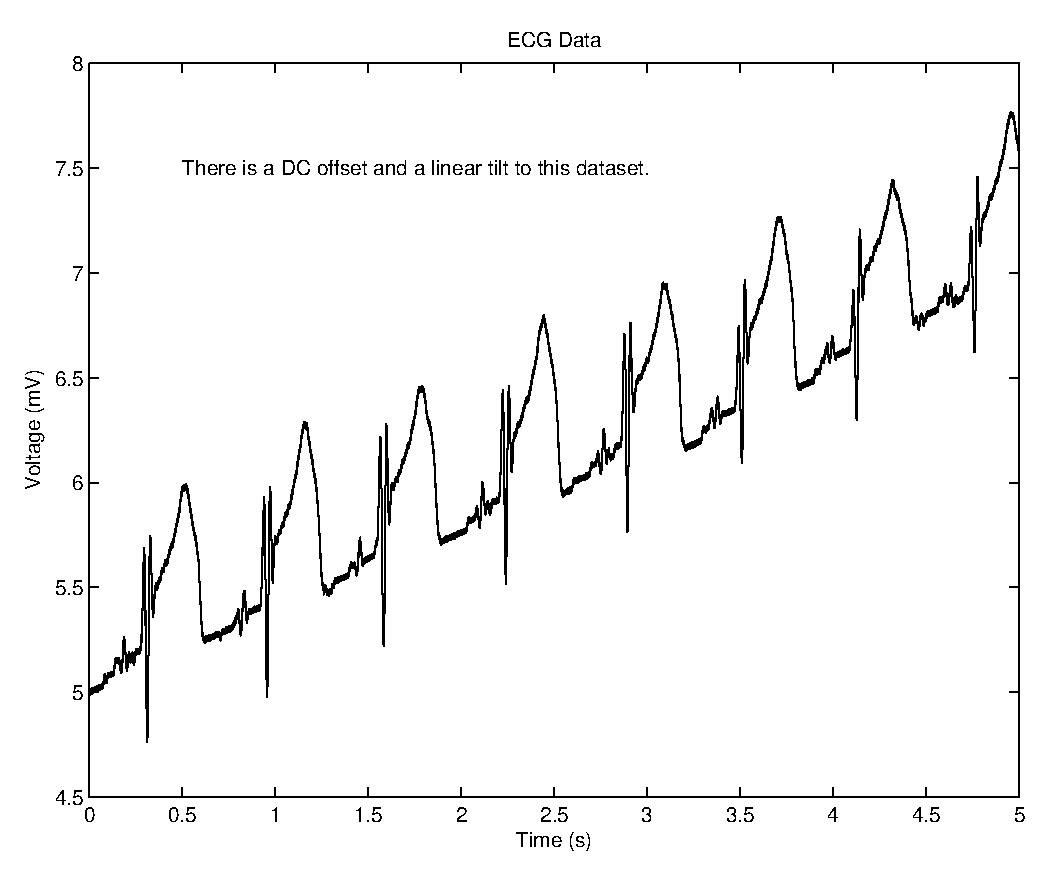
\includegraphics[width=0.5\linewidth]{ecg_data/ecg_dat.eps}
\end{center}

Differences between signals:
\begin{enumerate}
\item DC offset
\item Linear tilt through time
\end{enumerate}

After removing these artifacts (subtracting a linear fit of the data using the \verb+polyfit+ command), the following signal is generated:

\begin{center}
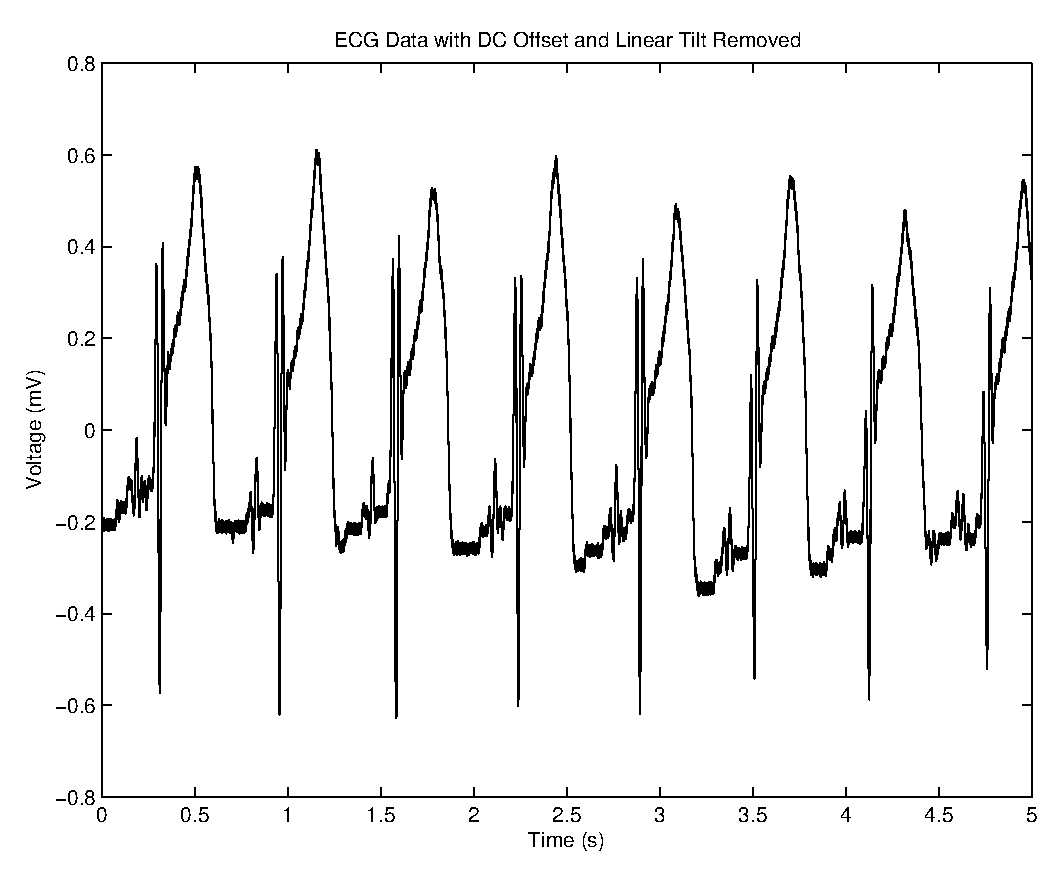
\includegraphics[width=0.5\linewidth]{ecg_data/ecg_dat_clean.eps}
\end{center}

The corresponding FFTs of the tilted and filtered data are shown below:

\begin{center}
\begin{tabular}{cc}
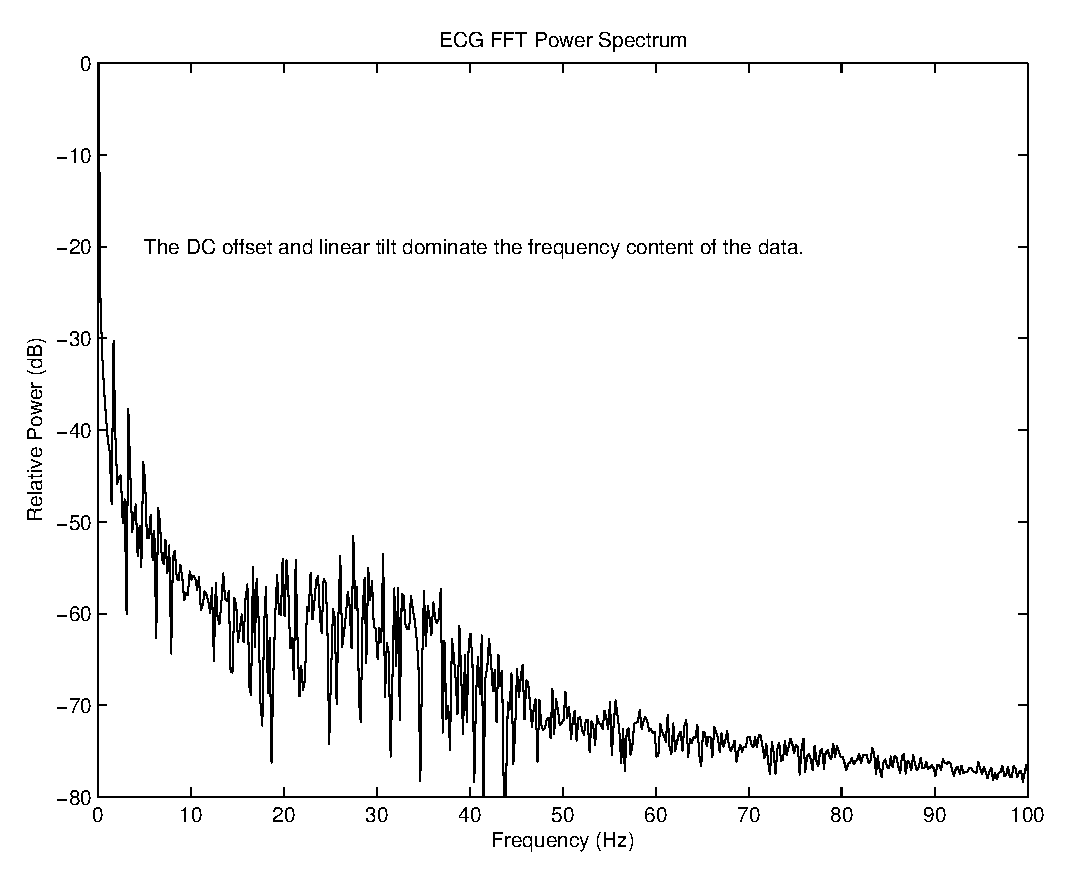
\includegraphics[width=0.5\linewidth]{ecg_data/ecg_fft.eps} &
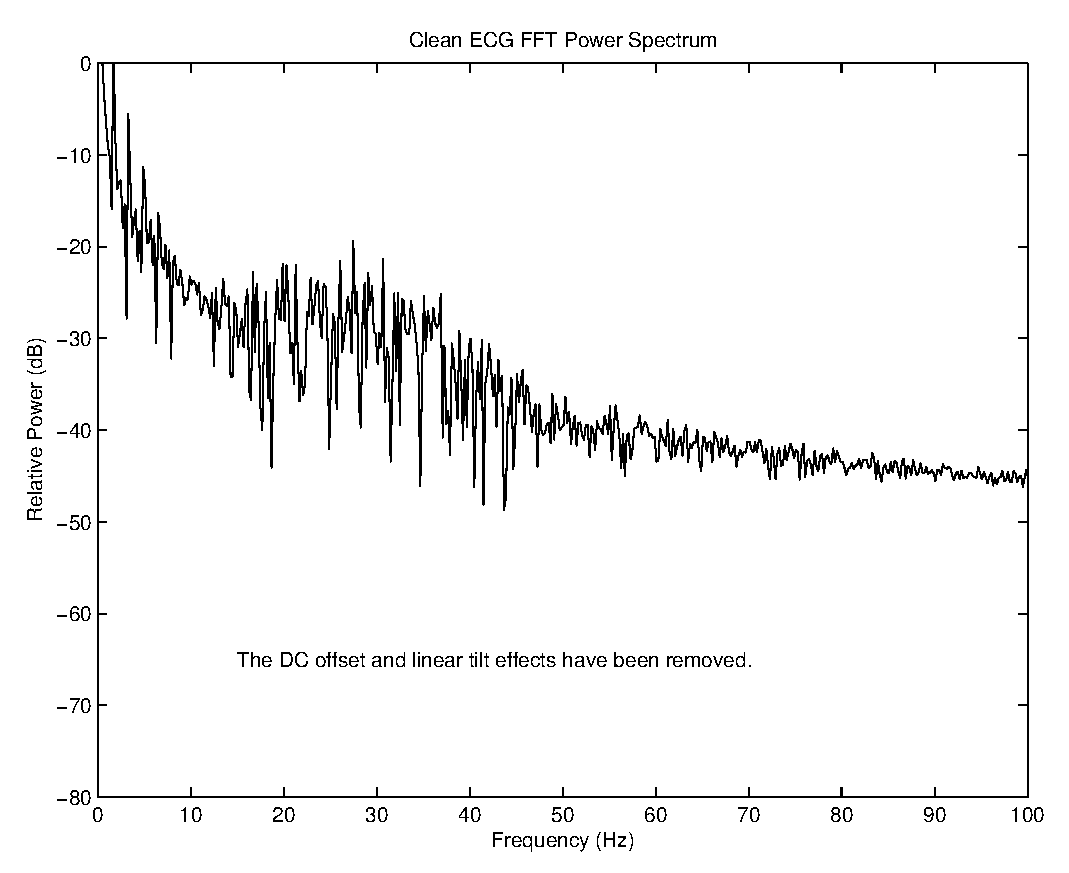
\includegraphics[width=0.5\linewidth]{ecg_data/ecg_fft_clean.eps} \\
\end{tabular}
\end{center}

Looking at the filters ECG signal, we can see that most of the energy is still
concentrated in the low, near-DC range, with the higher-frequency components of
the ECG signal ranging from 15-50 Hz (qualitative observation of the power
spectrum).  The code to read in the binary data, remove the tilt (one
time-domain approach; could use frequency domain filtering approach too), and
computing the FFT are shown below:

\begin{verbatim}
% load in the data
fid = fopen('BME154L_S10_PS7_ECG.dat','r');
data = fread(fid,'float32');
fclose(fid);
t = data(1:2:end);
ecg = data(2:2:end);
clear data
figure(1);
plot(t,ecg);
xlabel('Time (s)');
ylabel('Voltage (mV)');
title('ECG Data');
text(0.5,7.5,'There is a DC offset and a linear tilt to this dataset.');
print -deps2 ecg.eps

% compute FFT
fs = 1/mean(diff(t));
ft = fft(ecg);
f = linspace(-fs/2,fs/2,length(ft));
figure(2);
plot(f,fftshift(20*log10(abs(ft)./max(abs(ft)))));
axis([0 100 -80 0]);
xlabel('Frequency (Hz)');
ylabel('Relative Power (dB)');
title('ECG FFT Power Spectrum');
text(5,-20,'The DC offset and linear tilt dominate the frequency content of the data.');
print -deps2 ecg_fft.eps

% remove DC offset and linear tilt from data
p = polyfit(t,ecg,1); % fit a line to the data
artifact = p(1)*t + p(2);
clean_ecg = ecg - artifact;
figure(3);
plot(t,clean_ecg);
xlabel('Time (s)');
ylabel('Voltage (mV)');
title('ECG Data with DC Offset and Linear Tilt Removed')
print -deps2 ecg_clean.eps

% compute clean FFT
ft_clean = fft(clean_ecg);
figure(4)
plot(f,fftshift(20*log10(abs(ft)./max(abs(ft_clean)))));
axis([0 100 -80 0]);
xlabel('Frequency (Hz)');
ylabel('Relative Power (dB)');
title('Clean ECG FFT Power Spectrum');
text(15,-65,'The DC offset and linear tilt effects have been removed.');
print -deps2 ecg_fft_clean.eps
\end{verbatim}

Next we can evaluate the effect of downsampling the datasets (Figure~\ref{fig:ecg_downsample}).

\begin{figure}[h!]
$\begin{array}{ccc}
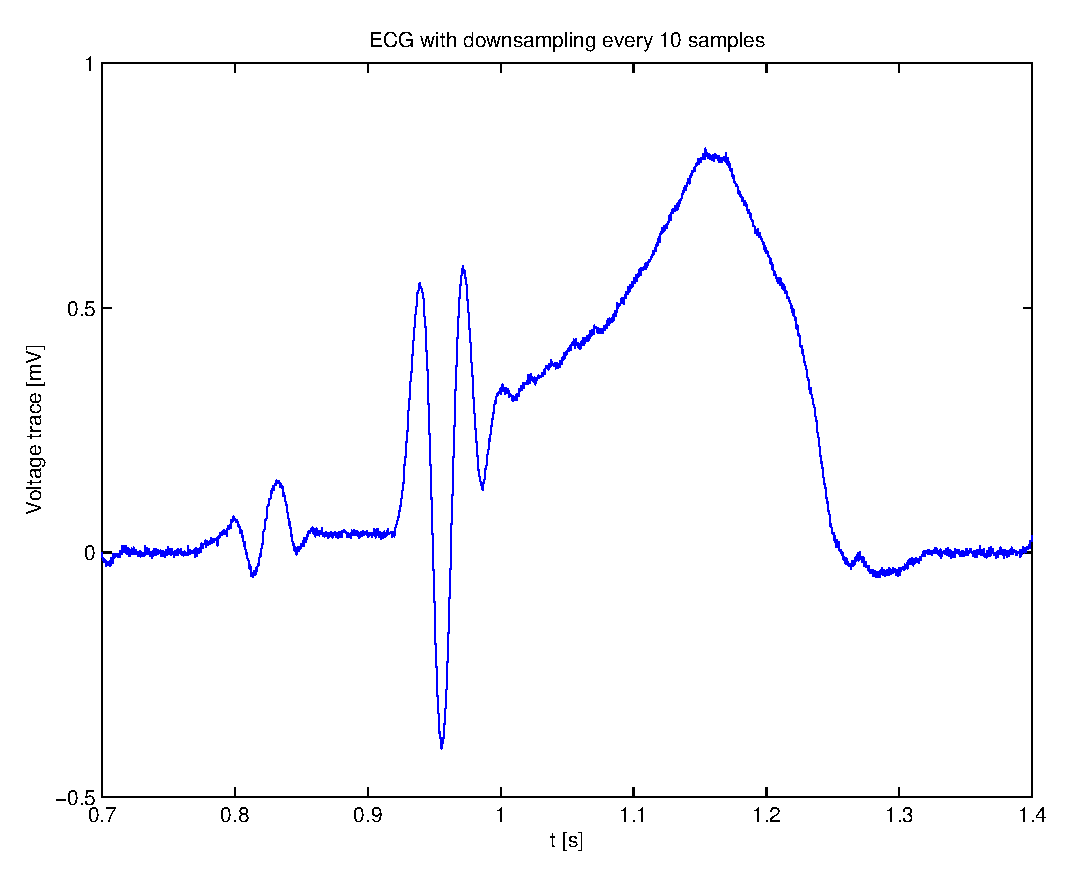
\includegraphics[width=2in]{ecg_data/downsample_10.eps} &
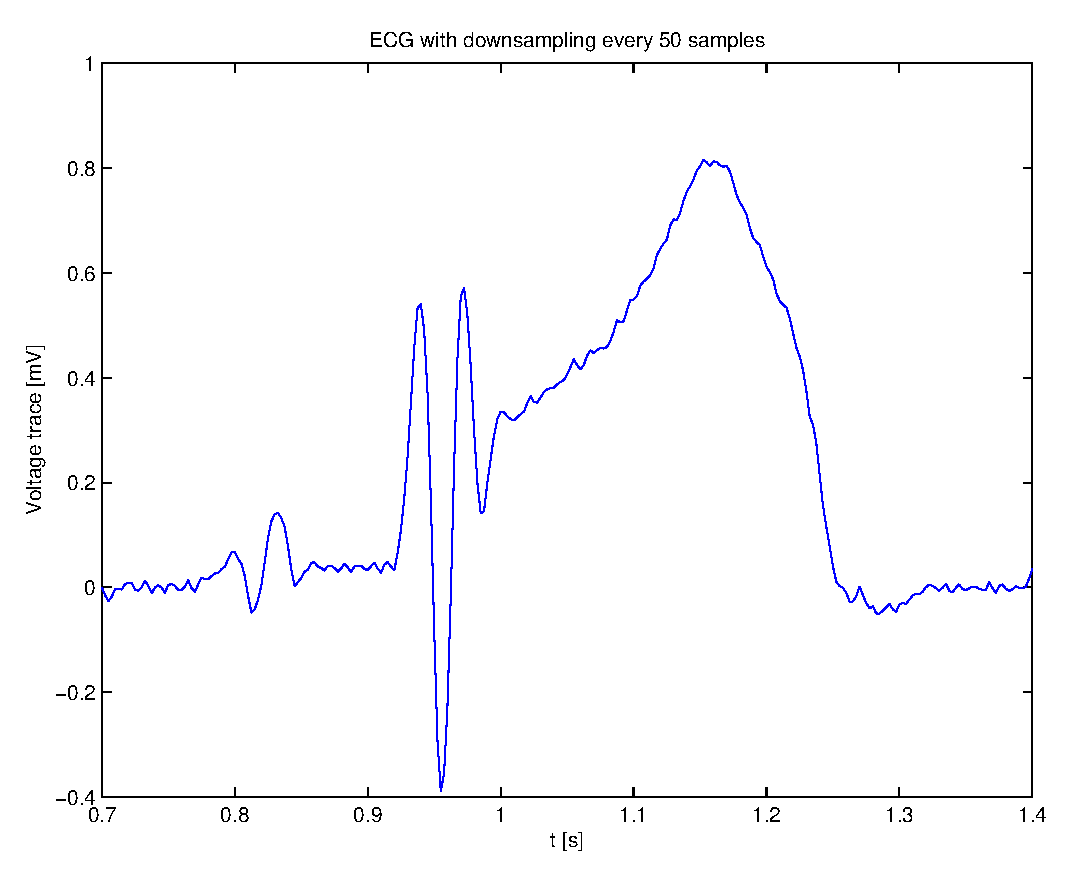
\includegraphics[width=2in]{ecg_data/downsample_50.eps} &
\includegraphics[width=2in]{ecg_data/downsample_100.eps} \\
\includegraphics[width=2in]{ecg_data/downsample_200.eps} &
\includegraphics[width=2in]{ecg_data/downsample_500.eps} &
\includegraphics[width=2in]{ecg_data/downsample_1000.eps} 
\end{array}$
\caption{Looking at the datasets, we can see that between skipping every 100
and 200 samples that the signal integrity has been preserved; more aggressive
downsampling leads to lost information in the signal morphology.}
\label{fig:ecg_downsample}
\end{figure}

100 samples, the shape of the signal is preserved and we can have confidence
that the peaks of the signal are very close to what we would expect. When we
sample ever 200 samples, we can already see (particularly in the shape of the
first peak) that there is some corruption of peak location. Especially with an
ECG signal, this type of corruption can lead to mistakes in diagnosis and
should really be prevented. We can see aliasing clearly in the every-500 and
every-1000 case because we miss one and two of the peaks of the QRS complex
respectively, lowering the 'frequency' we see in that area. Thus, we might
suspect that an adequate sampling frequency for this signal that would
correspond to minimizing the noise but maximizing the signal fidelity might be
around sampling every 150 samples, which would correspond to the following
sampling frequency as shown below:

\begin{equation} f_s = \frac{1}{t(151)-t(1)} = 133.33 ~\textrm{Hz} \end{equation}

As we know from Nyquist, this frequency will correspond to approximately twice
the maximum frequency seen in the signal (if it is the minimum sampling
frequency), so the maximum frequency content of the signal is likely around
66.7 Hz.  Those coincides well with the observations we made on the filtered
ECG power spectrum.

We can also find that the data acquisition sampling frequency was 150 times the
minimum sampling frequency (which makes sense because we identified skipping
150 samples as being optimal).

Power spectra of the downsampled ECG data have not been presented, but were
expected to be generated as done for the original ECG signals.
